\documentclass[Royal,times,sageh]{sagej}

\usepackage{moreverb,url,natbib, multirow, tabularx}
\usepackage[colorlinks,bookmarksopen,bookmarksnumbered,citecolor=red,urlcolor=red]{hyperref}


% Pandoc citation processing

\usepackage{tikz}
\usetikzlibrary{positioning}
\usepackage{threeparttable}
\usepackage{booktabs}
\usepackage{dcolumn}
\usepackage{bm}
\usepackage{mathtools}
\usepackage{amssymb}
\usepackage{amsmath}
\usepackage{amsthm}
\usepackage{subfig}
\DeclareMathOperator{\E}{\mathbb{E}}
\DeclareMathOperator{\Var}{\mathrm{Var}}
\DeclareMathOperator{\Cov}{\mathrm{Cov}}
\DeclareMathOperator*{\argmax}{arg\,max}
\DeclareMathOperator*{\argmin}{arg\,min}
\mathtoolsset{showonlyrefs}
\newtheorem{hyp}{Hypothesis}
\newtheorem{subhyp}{Hypothesis}[hyp]
\renewcommand\thesubhyp{\thehyp.\alph{subhyp}}
\usepackage{booktabs}
\usepackage{longtable}
\usepackage{array}
\usepackage{multirow}
\usepackage{wrapfig}
\usepackage{float}
\usepackage{colortbl}
\usepackage{pdflscape}
\usepackage{tabu}
\usepackage{threeparttable}
\usepackage{threeparttablex}
\usepackage[normalem]{ulem}
\usepackage{makecell}
\usepackage{xcolor}


\begin{document}

\title{Examining pseudo opinions and fictitious issues in online
surveys}

\runninghead{Andersen \emph{et al}.}

\author{H. K. Andersen*\affilnum{1}, J. Mayerl\affilnum{1}, F.
Wolter\affilnum{2}, J. Junkermann\affilnum{3}}

\affiliation{\affilnum{1}{Institute of Sociology, Chemnitz University of
Technology, Chemnitz, Germany}\\\affilnum{2}{Department of Sociology,
Universität Konstanz, Konstanz, Germany}\\\affilnum{3}{Institute of
Sociology, Johannes Gutenberg Universität Mainz, Mainz, Germany}}

\corrauth{Henrik Kenneth Andersen, Institute of Sociology, Chair for
Sociology with a Focus on Empirical Social Research, Chemnitz University
of Technology, Thüringer Weg 9, 09126 Chemnitz.}

\email{\href{mailto:henrik.andersen@soziologie.tu-chemnitz.de}{\nolinkurl{henrik.andersen@soziologie.tu-chemnitz.de}}}

\begin{abstract}
xxx
\end{abstract}

\keywords{pseudo opinions; ficitious issues; survey research; online
surveys; response latencies}

\maketitle

\renewcommand{\thefootnote}{\arabic{footnote}}

\hypertarget{introduction}{%
\section{Introduction}\label{introduction}}

Online surveys have grown increasingly popular in academic contexts in
the social sciences \citep{Bandilla2016, Silber2013}. The reasons why
are clear: they are comparatively cheap, can be conducted quickly and
they make it possible to skip the data entry phase. Furthermore, there
are a number of studies that propose that the quality of data collected
in online surveys is actually better than in other modes like telephone
and mail surveys. This proposition is often based on the argument that
online surveys lessen social desirability pressures, and the observation
that online surveys tend to produce lower item nonresponse rates and
less dropouts \citep{Shin2011}.

On the other hand, there are issues of coverage and representativeness
associated with typically non-probability sampled online surveys.
Furthermore, are lower item nonresponse rates necessarily an indicator
of higher quality data? If the answers being supplied are nonsense, are
they really preferable to missing values? Exactly this is the concern
some have with online surveys
\citep{Leiner2019, Kaminska2010, Vannette2014}. Namely, online surveys
often employ `professional' panelist who receive incentives for taking
part \citep{Stocke2006}. They are motivated by monetary concerns or a
`work-like' desire to fulfill their obligations \citep{Silber2013}.
Simple quality control measures are typically used by panel operators to
filter out respondents that provide obviously poor-quality data, meaning
panelists are incentivized to make it to the end of the survey without
skipping too many questions or giving non-substantive (``don't know'')
responses.

These issues are made even more prickly by the fact that online surveys
provide less control over the `interview' situation and it is more
difficult to tell whether a respondent is distracted, has understood the
question properly, or is giving misleading or meaningless data
maliciously \citep{Leiner2019}. This means that some methods of
assessing the quality of data are unavailable for online surveys, i.e.,
interviewer recorded impressions (``Did the respondent understand the
question?''). Others, like post hoc data cleaning methods, i.e.,
removing fast respondents or individual responses, identifying and
removing straight-liners, etc., are available, but can inadvertently
introduce new biases to the data \citep{Leiner2019}. One promising
approach is to assess the degree of mental elaboration expended for a
response, which can be done non-reactively with the use of response
latencies \citep[reactive methods may try to directly assess the
respondent's motivation and opportunity by asking directly about
them,][]{Mayerl2008, Stocke2006}. Namely, if we can assess the effort
the respondent is willing to expend to answer a survey question, we can
begin to get an idea of the quality of their answer.

What make response latencies difficult to interpret is that they can
indicate both the degree of mental elaboration, or the accessibility of
the attitude object \citep{Stocke2004c}. I.e., if we observe a fast
response, we cannot be sure whether it was because the respondent had a
salient attitude ready to express spontaneously, or whether the
respondent was lacking either motivation or opportunity and turned to
some response set to avoid putting in the effort to properly answer the
question (e.g., satisficing). This is particularly troubling because
they suggest two completely different conclusions. Namely, accessible
attitudes are typically strong ones, so fast responses motivated by an
accessible attitude will likely possess high (predictive) validity. On
the other hand, fast responses due to satisficing can be completely
independent of the question content, indicating poor validity.

In this article, we propose using \textit{fictitious issues}, i.e.,
questions about nonexistent topics, together with response latencies to
assess the quality of data gathered in online surveys. With fictitious
issues, we can be sure that the respondent does not have an accessible
attitude --- how could they when the attitude object does not exist?
Therefore, fast or slow responses can logically only be a sign of the
cognitive effort a respondent is willing to exert, either to generate an
ad hoc attitude or come to the honest conclusion that they ``don't
know''.

In this context, the question of whether missing values are preferable
to deliberate responses to fictitious issues is open. The imputed
meaning hypothesis states that, when faced with unfamiliar or obscure
topics, survey respondents attempt to generate an ad hoc opinion by
searching for cues and abstracting the question to a more general level
\citep{Sturgis2010}. If this is the case, then these `pseudo opinions',
as they are sometimes called, can be seen as valid measures of
generalized attitudes with which the respondent connects the survey
item. If this is seen as desirable by the researcher, pseudo opinions
may be preferable to missing values. If, on the other hand, the primary
interest is the specific attitude object, perhaps because generalized
attitudes are not expected to possess predictive validity, then pseudo
opinions should be avoided. To investigate this issue, we perform two
split ballot experiments: one in which we vary the presence of an
explicit ``don't know'' category, and another in which we instruct the
respondents to either answer spontaneously or deliberately.

We proceed as follows: xxx

\hypertarget{background}{%
\section{Background}\label{background}}

There is debate surrounding the quality of online surveys compared to
more traditional personal interviews and mail-in surveys. On the one
hand, it has been observed that online surveys tend to lessen the impact
of social desirability bias due to the anonymity the mode affords
\citep{Silber2013, Chang2009, Kreuter2008, deLeeuw2005}. Likely for the
same reason, online surveys also tend to produce lower item nonresponse
rates than traditional surveys \citep{Shin2011}; the increased anonymity
may make respondents more open to revealing sensitive information like
their income. On the other hand, web surveys employing `professional'
\footnote{Here `professional' refers to the pool of reoccurring
  participants in surveys who take part in exchange for money or other
  incentives, whether or not is is the person's main source of income.}
panelists are thought to lead to other response effects, notably
satisficing. Namely, panelists are motivated primarily by monetary
incentives; they are less likely to be intrinsically motivated out of
interest for the survey topic \citep{Silber2013}, or due to their
positive attitude towards surveys in general
\citep{Stocke2004a, Stocke2004c}.

Satisficing \citep{Krosnick1991, Roberts2019} in the context of surveys
refers to a set of strategies employed by respondents who are
\emph{weakly motivated}, \emph{lacking opportunity} (i.e., time
pressure), or both, to get through the survey with as little effort as
necessary \citep{Krosnick1991, Roberts2019}. That is, a popular model of
response behaviour encompasses four stages: (1) reading and
understanding the question, (2) retrieving relevant information from
memory, (3) forming a judgment and (4) translating the judgment to fit
one of the available response categories
\citep{Roberts2019, Tourangeau2000}. So-called ``weak'' satisficing
refers to responses that result when a respondent goes through all four
of the stages but in a cursory manner, leaving room for cognitive biases
(such as acquiescence, primacy, etc.). The respondent may begin to
search their memory for salient attitudes or relevant information in
order to form an ad hoc judgment, but they end the process once a
``first-best'' or satisfactory result is reached. In other words,
instead of optimizing their responses by attempting to consider all
relevant information and perspectives, they gather some salient impulses
and cut the process off. So-called ``strong'' satisficing, on the other
hand, refers to responses in which the respondent skips either the
information retrieval or judgment formation stages \citep{Vannette2014}.
That is, the respondent reads and comprehends the question and forms an
immediate response without attempting to form a connection between the
question and stored information and memories. If the respondent is
unable to intuit any easy cues for an ``effortless'' response
\citep{Roberts2019, Leiner2019}, they may either select a response at
random (``mental coin flip'') or skip the question or provide another
form of nonsubstantive response \citep[e.g., ``don't
know'',][]{Vannette2014}. Thus, the \emph{difficulty of the task} is
often mentioned as the third component that is said to determine the
likelihood of satisficing, or rather the extent to which a respondent
moves from optimizing to weak to even strong satisficing. I.e.,
\(P(\text{satisficing}) = \text{task difficulty}/(\text{motivation} \times \text{opportunity})\)
\citep{Roberts2019}. Still another form of response behaviour can be
distinguished from strong satisficing in which the respondent does not
even attempt to comprehend the question, thereby skipping even the first
stage. This is sometimes referred to as ``mindless'' responding
\citep{Vannette2014} in that the respondent's attention is not focused
on the survey questions.

As such, we can think of the quality of a response on a continuum from
optimizing to mindless responding, with weak and strong satisficing
somewhere in the middle, see Figure \ref{fig:continuum}. Where a
respondent finds themselves on this continuum is determined to a large
extent by their motivation and opportunity, as well as the difficulty or
burden of the task.

\begin{figure}
\centering
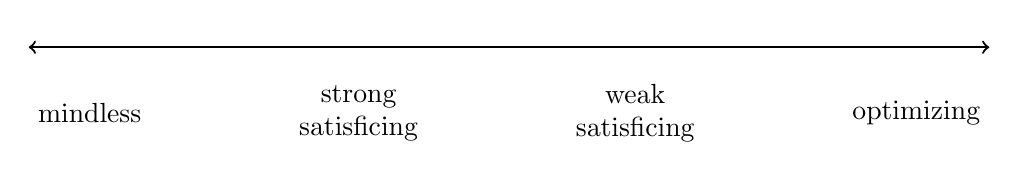
\begin{tikzpicture}[every pin/.append style={text width=5em},
    every pin edge/.style={draw},node distance=5em]
\begin{scope}[local bounding box=bb]
\node[below, align=center](m){mindless};
\node[right=of m, align=center](ss){strong\\satisficing};
\node[right=of ss, align=center](ws){weak\\satisficing};
\node[right=of ws, align=center](o){optimizing};
\end{scope}
\draw[thick, <->] 
 ([yshift=1em]bb.north west) node[above right]{}
 -- ([yshift=1em]bb.north east) node[above left,align=center]{};
\end{tikzpicture}
\caption{Quality of responding continuum}
\label{fig:continuum}
\end{figure}

\hypertarget{expected-behavioural-outcomes}{%
\subsection{Expected behavioural
outcomes}\label{expected-behavioural-outcomes}}

We are primarily interested in two behavioural outcomes when it comes to
responses: (1) substantive ``pseudo opinions'' and (2) nonsubstantive
responses, which are given by the respondent selecting ``don't know'' or
skipping the question. Professional panelists, especially those who
habitually give poor quality answers, are de-incentivized to give
nonsubstantive responses, because an over-reliance on them could trigger
the panel operator's quality control mechanisms and have them removed
from the panel for future surveys (thereby cutting them off from the
monetary benefits). For this reason, even very weakly motivated
panelists will likely turn to other satisficing strategies besides
nonresponses in the form of ``don't know''. If satisficing
respondents\footnote{Throughout, we may, for the sake of expediency,
  refer to `satisficers' and `optimizers'. This should be taken as
  shorthand for 'a respondent that is currently, specific to one single
  survey item, satisficing/optimizing".} encounter a question with which
they are unfamiliar with, they may look to contextual hints to give a
spontaneous cue-driven response. However, this process will necessarily
be a form of satisficing, because (a) strictly speaking previous
memories and information concerning the attitude object cannot
exist\footnote{It is conceivable that the respondent could mistake the
  fictitious content for some existent one, but we assume this will
  happen infrequently, and that the likelihood of this mistake is not
  related to any of the other predictors of interest, so that they
  should be ignorable.} and (b) a drawn-out futile memory search defeats
the purpose of satisficing as a way to avoid effort. Mindlessly
responding-respondents\footnote{The respondents are of course not
  mindless; their current response behaviour may be taking place without
  much thought given to the question contents though.} who do not wish
to trigger quality control mechanisms will respond quasi-randomly using
effortless patterns and heuristics, but will tend not to rely overly on
the ``don't know'' category. For these reasons, we believe that
satisficing respondents will tend towards substantive answers to
unfamiliar of wholly fictitious topics out of fear of triggering quality
control mechanisms.

On the other hand we have optimizing respondents. These will tend to be
respondents that are (currently) motivated and have sufficient
opportunity for deliberate thought. One characteristic that is tied to
motivation is often cited as the respondent's attitudes towards surveys
\citep{Stocke2004a, Stocke2004c}. Respondents that find surveys
generally useful and accurate tend to be motivated to provide high
quality responses. Ability is often tied to cognitive abilities (e.g.,
understanding the question, although this is presumably less of an issue
for professional panelists), or time pressure. Respondents that lack
time pressure have the luxury of deliberating on a question before
providing an answer. It is unclear how optimizing respondents behave
towards fictitious or obscure topics. \citet{Sturgis2010} suggests that
respondents attempt to impute a meaning when faced with an unfamiliar
topic, by looking for clues in the question and extrapolating to some
seemingly related attitude object. On the other hand, optimizing
respondents driven by a belief that surveys are useful and helpful in
guiding policy may try to avoid reporting an opinion on something they
do not feel sufficiently familiar with.

Based on these points, it is unclear whether optimizing respondents will
tend towards imputed-meaning driven pseduo-opinions or nonsubstantive
``don't know'' avoidance. The imputed meaning hypothesis is persuasive,
but there is a lack of empirical evidence for it. In online surveys
employing professional panelists, the idea that many or even most
respondents consider their responses carefully is implausible. Without
taking the motivation and opportunity of a respondent into account, the
simple fact that a respondent gave a substantive response could just as
well be evidence of satisficing behaviour ranging from simple heuristics
to a mental coin flip.

\hypertarget{indicators-of-satisficing-and-optimizing}{%
\subsection{Indicators of satisficing and
optimizing}\label{indicators-of-satisficing-and-optimizing}}

It is very easy to record passive response times in online surveys.
Online survey software often automatically records the response time per
page or the whole survey completion time. There are, however, drawbacks
to these measures. For example, if less motivated respondents tend to be
more distracted, then the level of distractedness will be a confounder
of the effect of motivation on responses. Thus, completion times may not
be an accurate indicator of effort. Furthermore, while per-page
responses and completion times can reveal a tendency, they assume the
motivation and opportunity of the respondent is constant throughout the
survey (or within one survey page). Surely the contents of the item can
have an effect on the motivation and/or opportunity. Therefore, we turn
to per-item response latencies in the hopes of getting a more precise
measure of the effort put in by the respondent, thereby also allowing us
to better assess the relationship between effort and responses.

Per-item response latencies (i.e., for each individual question a
response time is recorded) have the benefit of being specific to a
clearly defined question content. If the content of the question has an
impact on the motivation and/or opportunity, we can hold this constant
by use of various methods (e.g., item dummies). Further, for each
respondent, we have multiple per-item response latency measurements.
This means we can examine the effect of the latencies on survey
behaviour in a multilevel framework. This gives us the added opportunity
to hold respondent-level characteristics (personality, reading speed,
internet connection, etc.) constant as well.

Both forms of satisficing, as well as mindless responding represent
strategies to reduce effort. As such, they should be associated with
faster response latencies, otherwise they lose their appeal: careful or
deliberate satisficing is an oxymoron. While it is typically the case
that fast responses can either be a sign of satisficing or mindless
responding on the one hand, or highly salient attitudes, on the other,
in the case of fictitious issues, they can only be a sign of the former.
Because the attitude object does not exist, there cannot exist salient
attitudes towards it. Based on the contextual clues surrounding the
fictitious issue, the respondent may be able to quickly impute a meaning
and give a response based on that understanding, but this is not a
characteristic of a high-quality answer. Fast substantive responses to
fictitious issues are either a sign that the respondent did not properly
read the question (and the answer is therefore independent of the
question contents) or the respondent read the question, quickly imputed
a meaning and gave an answer based on that understanding. But this is
practically the definition of satisficing; to come to the first-best
plausible response and move on. If the respondent was optimizing, they
would be tempted to verify if their gut-response is appropriate: e.g.,
``Do I really know what the `Coastal Aid Agency' does, and whether I
support those goals?''.

Optimizers, on the other hand, are characterized by a willingness to
cooperate with what they perceive as the survey researcher's goals
\citep{Stocke2004a}. In the context of fictitious issues, this could
express itself in at least two ways: (1) the respondent recognizes that
the question contents are unfamiliar and answer truthfully with ``I
don't know''. Unlike habitual satisficers, they have nothing to fear
about giving nonsubstantive responses. (2) The respondent attempts to
``impute a meaning'' and offers a response in line with what they
perceive the question contents concern. The behaviour of the respondent
may be misguided, but it is still a sign of a high quality response in
the sense that the respondent had ample opportunity to give up and give
either a non-substantive or meaningless response but they did not.
Because of this ambiguity, we investigate in an exploratory fashion
whether optimizers tend to give substanitve or nonsubstantive responses
when faced with unfamiliar topics by default.

\hypertarget{analysis}{%
\section{Analysis}\label{analysis}}

\hypertarget{data-and-variables}{%
\subsection{Data and variables}\label{data-and-variables}}

\begin{table}

\begin{threeparttable}
\caption{\label{tab:unnamed-chunk-1}\label{tab:freqs}Responses to existent institutions in percent}
\centering
\begin{tabular}[t]{lrrrrrrrr}
\toprule
  & BW & DWB & UN & GP & BKA & RLF & KAF & IPCC\\
\midrule
negative & 36.80 & 9.55 & 21.43 & 22.59 & 19.10 & 15.76 & 12.73 & 24.22\\
positive & 56.37 & 86.10 & 71.43 & 71.20 & 72.13 & 42.62 & 62.73 & 44.18\\
continue & 5.20 & 1.79 & 4.50 & 4.43 & 5.43 & 15.45 & 10.95 & 10.40\\
don't know & 1.63 & 2.56 & 2.64 & 1.79 & 3.34 & 26.16 & 13.59 & 21.20\\
\bottomrule
\end{tabular}
\begin{tablenotes}
\small
\item [] BW: German Armed Forces (Bundeswehr), DWB: Doctors without Boarders, UN: United Nations, GP: Greenpeace, BKA: German Federal Criminal Police (Bundeskriminalamt), RLF: Rosa-Luxemburg-Foundation, KAF: Konrad-Adenauer-Foundation, IPCC: Intergovernmental Panel on Climate Change
\end{tablenotes}
\end{threeparttable}
\end{table}

\begin{table}

\begin{threeparttable}
\caption{\label{tab:unnamed-chunk-1}\label{tab:freqs_fi}Responses to fictitious institutions in percent}
\centering
\begin{tabular}[t]{lrrrrrr}
\toprule
  & EC & CAA & PETI & GNF & HSF & WSA\\
\midrule
negative & 15.92 & 10.95 & 15.37 & 22.28 & 10.48 & 13.59\\
positive & 58.54 & 48.06 & 28.34 & 22.59 & 12.97 & 26.48\\
continue & 8.54 & 11.72 & 18.48 & 17.86 & 30.90 & 21.35\\
don't know & 17.00 & 29.27 & 37.81 & 37.27 & 45.65 & 38.59\\
\bottomrule
\end{tabular}
\begin{tablenotes}
\small
\item [] EC: Environmental Court, CAA: Coastal Aid Agency, PETI: Prague Energy Transition Initiative, GNF: German Nuclear Forum, HSF: Herbert-Schmaar-Foundation, WSA: World Space Agency
\end{tablenotes}
\end{threeparttable}
\end{table}

\begin{figure}

{\centering \subfloat[\label{fig:raw}Raw latencies\label{fig:response-latency-plots-1}]{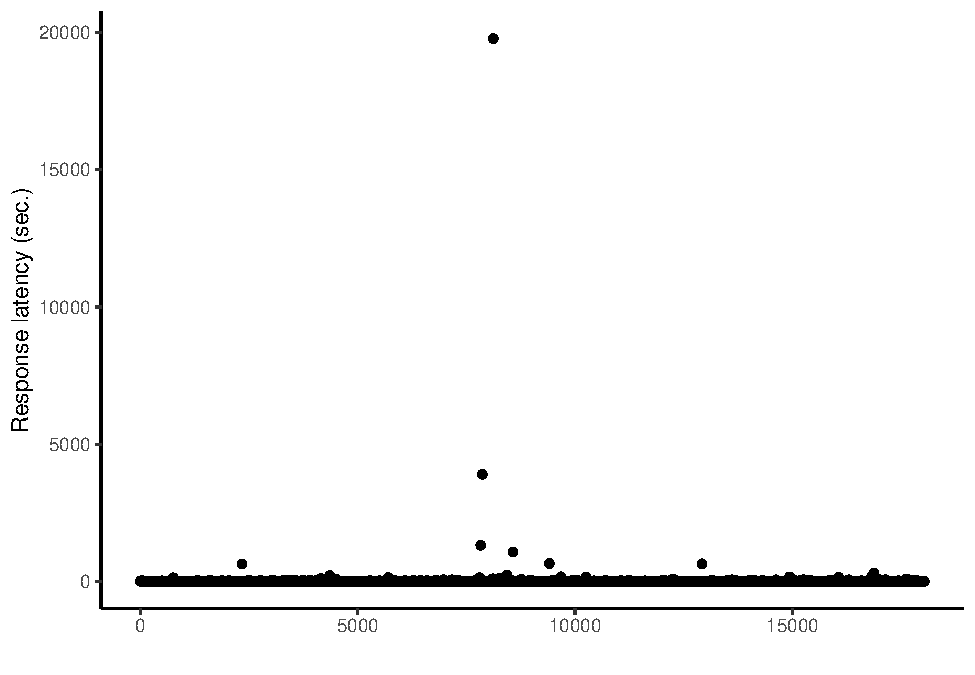
\includegraphics[width=0.4\linewidth]{article_files/figure-latex/response-latency-plots-1} }\subfloat[\label{fig:invalid}Valid latencies less than 2,000 sec.\label{fig:response-latency-plots-2}]{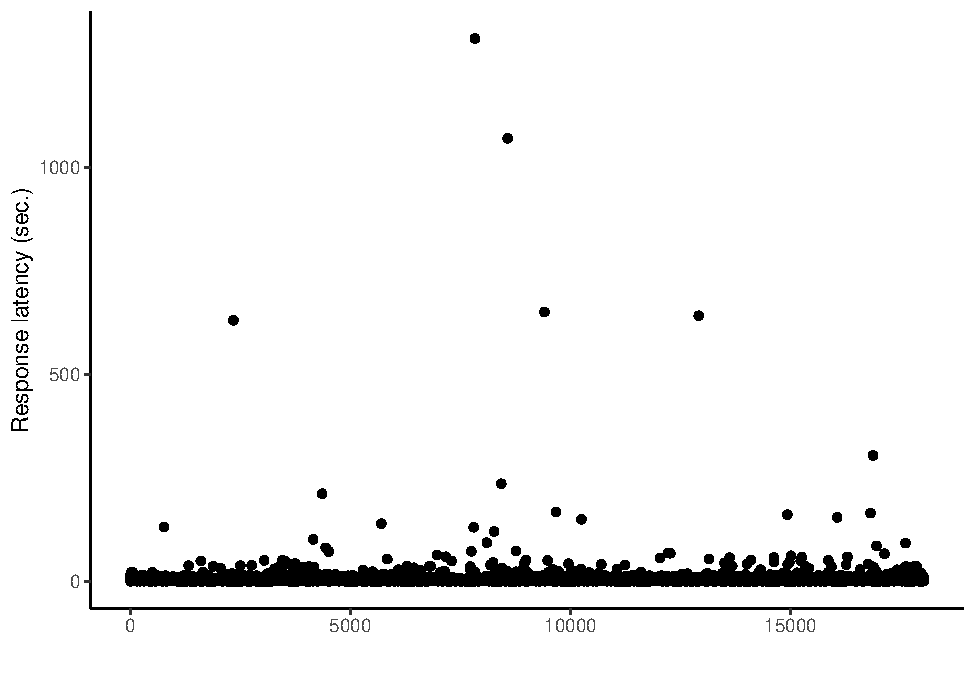
\includegraphics[width=0.4\linewidth]{article_files/figure-latex/response-latency-plots-2} }\newline\subfloat[\label{fig:outlier}Latencies less than 2 sd above the mean\label{fig:response-latency-plots-3}]{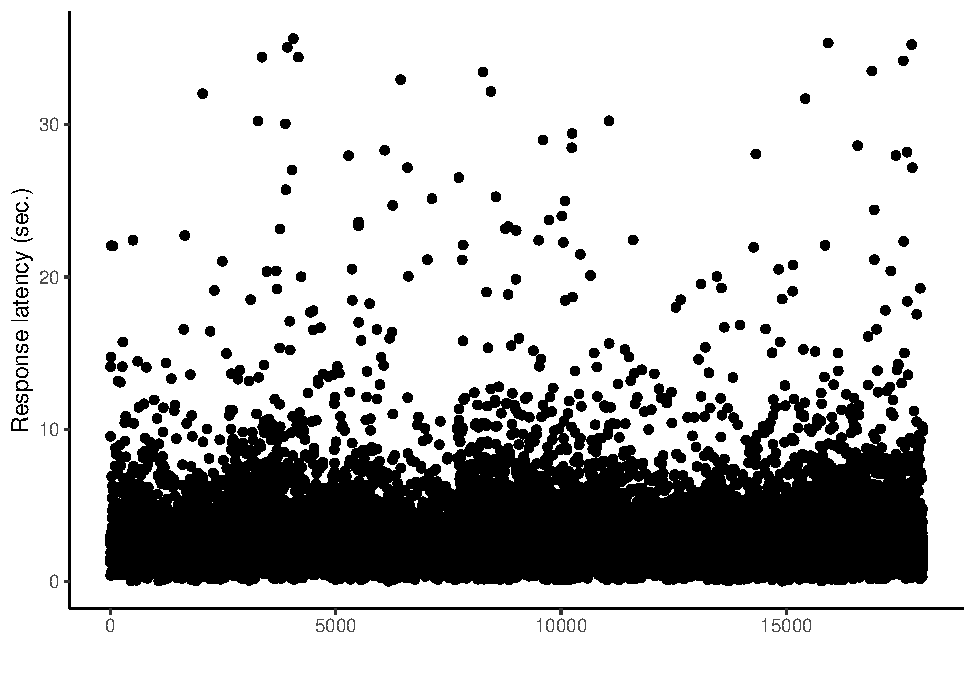
\includegraphics[width=0.4\linewidth]{article_files/figure-latex/response-latency-plots-3} }

}

\caption{\label{fig:rls}Response latency treatment}\label{fig:response-latency-plots}
\end{figure}

We conducted an online survey using an online access panel provided by
an online panel provider from 16th to 25th August 2019. The target
population was defined as adults between the age of 18 and 69 years with
quotas for age and sex in place to ensure the sample was representative
of the target population on those characteristics. The respondents were
recruited from the provider's pool of `professional' respondents.

The pseudo opinions portion of the study consisted of a question battery
in which the respondents were asked using a binary scale to give us
their opinion (mostly positive vs.~mostly negative) on 14 different
organizations and institutions. These covered eight which truly existed,
and six which were fabricated by us. This part of the study encompassed
a split of 1288 randomly chosen respondents out of the full sample of
3,044. Within the group of these 1288 respondents, two randomized
experiments were conducted in which, firstly, 645 respondents were
presented with an explicit ``don't know'' category throughout, while for
the remaining 643 there was no explicit ``don't know'' category
available. For these respondents, the option was available for them to
simply click on ``continue'' to skip the question. Secondly, within the
implicit ``don't know'' group, 322 were given the instructions to think
carefully and provide the most accurate answers possible, and 321 were
given the instructions not to think too long, and to provide spontaneous
answers. In the explicit ``don't know'' group, 322 were given the
accuracy instructions and 323 the speed instructions.

As noted, we asked respondents to tell us their opinion on a binary
scale (``mostly positive'' vs.~``mostly negative'') towards a range of
organizations and institutions.\footnote{The question text read: ``For
  the following questions, we are interested in your opinions towards
  different organizations and institutions. We would like to know
  whether you find these organizations generally good or bad.''} In
total, respondents were presented with 14 of these organizations, eight
of which truly exist (e.g., Doctors Without Boarders, Greenpeace, the
German Armed Forces), six of which were fabricated. These were the
``Environmental Court'' (EC), the ``Coastal Aid Agency'' (CAA), the
``Prague Energy Transition Initiative'' (PETI), the ``German Nuclear
Forum'' (GNF), the ``Herbert-Schmaar-Foundation'' (HSF) and the ``World
Space Agency'' (WSA). Table \ref{tab:freqs} shows the responses to the
existent institutions and organization, while Table \ref{tab:freqs_fi}
shows the responses to the fictitious ones. The ``don't know'' category
was available only to those respondents in the ``explicit don't know''
experimental group.

\hypertarget{operationalization}{%
\subsection{Operationalization}\label{operationalization}}

Response latencies needed to be treated before analysis, see Figure
\ref{fig:rls}. Panel \ref{fig:raw} shows the original, raw latencies
before any treatment. Several measurements stand out as being extremely
long. The longest response latency was nearly 20,000 seconds or 5.6
hours. Still others were upwards of 2,000 seconds or 33.3 minutes. These
cannot possibly be thought of as valid responses (in the sense that they
would tell us anything about underlying cognitive processes); very
likely the respondent interrupted the survey and came back to it much
later. Panel \ref{fig:invalid} shows the latencies after eliminating
those that were longer than 2,000 seconds. Panel \ref{fig:outlier} shows
a second treatment step in which latencies two standard deviations above
the mean (after removing latencies longer than 2,000 seconds) were
treated as outliers.

\hypertarget{method}{%
\subsection{Method}\label{method}}

We are interested in the probability of someone giving a substantive
response to a fictitious issue given the response latency (a measure of
one's current motivation and opportunity), and the experimental
conditions (speed vs.~accuracy and implicit vs.~explicit ``don't
know''). For the response latencies, we also include a squared term
which, in the case of a linear model, allows for nonlinear effects. In
the nonlinear probit model we use here, it allows for effects that are
not monotonic (they do not have to either increase or decrease over all
values of the independent variable, but can change direction).

The dependent variable is a binary outcome (nonsubstantive,
substantive). The response latencies are continuous and vary across both
individuals and items, while the experimental conditions vary between
individuals but do not change within individuals. With a manageable
number of items, we can include dummy variables to control for the
item-specific effects, i.e., characteristics of particular items that
influence the way in which all respondents approach the question.

The unobserved effects probit model \citep{Wooldridge2002} lends itself
well to this setup. We can write the model as\\
\begin{align}
P(y_{ij} = 1| \bm{w}_{i}, \alpha_{i}) = \Phi(\bm{w}_{ij} + \alpha_{i}), \ j = 1, \ldots, J \label{eq:probit}
\end{align} where \(\Phi(\cdot)\) is the standard normal cumulative
distribution function.
\(\bm{w}_{ij} = (\bm{x}_{ij}, \bm{z}_{i}, \bm{\lambda}_{j})\) and
\(\bm{x}_{ij} = (\mathsf{rl_{ij}}, \mathsf{rl^{2}_{ij}})\) are the
response latency variables,
\(\bm{z}_{i} = (\mathsf{speed_{i}}, \mathsf{impdk_{i}})\) are the
experimental conditions and
\(\bm{\lambda}_{j} = (\lambda_{1}, \lambda_{2}, \ldots, \lambda_{J-1})\)
are item dummies (less the reference category).

Note that the first equality in Equation \eqref{eq:probit} is the
assumption of strict exogeneity, i.e., after controlling for the stable
individual differences in \(\alpha_{i}\), the predictors from other
points in time have no effect on the current point in time
\citep[p.~483]{Wooldridge2002}. This is why \(\bm{w}_{i}\) changes to
\(\bm{w}_{ij}\). We assume further that the only source of serial
correlation is \(\alpha_{i}\) so that once we have conditioned on it,
the errors are serially uncorrelated, and the likelihood function can be
derived as the product of the individual probabilities for \(y_{ij}\).

Correlations between the nonexperimental variables of interest (the
response latencies) and item characteristics (difficulty of the
question, wording effects, etc.) are controlled for by including the
item dummies in the equation. But we want to also allow (and control)
for correlations between the individual effects and the response
latencies. Importantly, we want to look at the speed of responses
relative to the person's average speed. That way we can assess within
individuals whether faster (satisficing) or slower (optimizing) than
average responses predict pseudo opinions. Essentially, we want to
specify a kind of binary outcome \textit{fixed effects} model in order
interpret the response latency effects as within-effects and ensure that
they are unbiased by between-person stable characteristics.

The \citet{Mundlak1978} approach to allowing for correlated individual
effects involves making assumptions about the distribution of the
individual effects \citep[p.~487]{Wooldridge2002}. Namely, we assume the
individual effects are normally distributed as \begin{align}
\alpha_{i} | \bm{w}^{*}_{i} & \sim \mathcal{N}(\psi + \bar{\bm{w}}^{*}_{i}\bm{\zeta}, \sigma^{2}_{\alpha})
\end{align} where \(\bm{w}^{*}_{i} = (\bm{x}_{i},\bm{z}_{i})\), i.e.,
\(\bm{w}_{i}\) without the item dummies.

That is, we assume
\(\alpha_{i} = \psi + \bar{\bm{w}}^{*}_{i}\bm{\zeta} + \upsilon_{i}\) so
that the error \(\upsilon_{i}\) is independent of the predictors. Now we
substitute this back into Equation \eqref{eq:probit} for \begin{align}
P(y_{ij} = 1| \bm{w}_{i}) = \Phi(\psi + \bm{w}_{ij}\bm{\beta} + \bar{\bm{w}}^{*}_{i}\bm{\zeta}), \ j = 1, \ldots, J.
\end{align} Essentially, we specify a multilevel model with random
intercepts (representing the individual effects) and include the
within-individual (or `cluster') means as a predictor of these random
intercepts. The cluster means are thus correlated with both the outcome
(the average outcome, so to speak) and the predictors in \(\bm{w}_{i}\).
This covariance is partialled out by including both in the regression so
that \(\bm{\beta}\) represent within-person effects that are
unconfounded by \(\alpha_{i}\)
\citep{Ruettenauer2019b, Hamaker2019, Wooldridge2002, Mundlak1978, Schunck2017}.

It is important to note that the item-invariant predictors
(\(\mathsf{speed_{i}}\), \(\mathsf{impdk_{i}}\)) can be included in
\(\bm{w}_{i}\) but their effects cannot be distinguished from
\(\alpha_{i}\) unless we assume that they are uncorrelated with
\(\alpha_{i}\) \citep[p.~488]{Wooldridge2002}. In other words, in the
vector \(\bm{\zeta}\) (the effects of the predictors on the random
intercepts), the coefficients for the item-invariant predictors are set
to zero. This is not problematic in our case because the item-invariant
predictors were fixed as a result of the randomized experimental
setting. In later models, when we include individual-level predictors
(e.g., sex, age, political orientation), we need to assume that they
were uncorrelated with the individual effects (a likely problematic
assumption), otherwise the effects will be biased.

\hypertarget{procedure}{%
\subsection{Procedure}\label{procedure}}

We proceed in a stepwise fashion. First (Model 1), we look at the
effects of the response latencies on the probability of a substantive
response, taking item- and individual-characteristics into account as
discussed above. Then we introduce the squared response latency term to
assess whether the effect changes direction over the values of
\(\mathsf{rl_{ij}}\). This we would expect if both satisficers (faster)
and optimizers (slower) tended towards substantive responses (albeit
for, we hypothesize, wholly different reasons). The correlated random
effects probit model described above involves including cluster means
for the item- and individual varying (sometimes called level 1)
predictors.

For the model with the quadratic response latency term (Model 2), we
therefore also include the squared within-individual response latency
\citep[as per][p.~97]{Schunck2017}.

Finally (Model 3), we introduce respondent-related characteristics to
examine their effects on the probability of a substantive response to a
fictitious issue. This is an exploratory step, as we do not have
concrete hypotheses regarding the respondent characteristics, and
furthermore it is unlikely that the effects can be given a causal
interpretation due to the potential confounding by other unobserved
respondent-related characteristics contained in \(\alpha_{i}\). The
respondent-level predictors are: sex (female, male), age (in years,
grand mean centered, range: (-26.753, 29.247), mean: 0, sd: 14.289),
need for social approval (three-item grand mean centered additive
index\footnote{Items: ``My decisions are sometimes unwise'', ``I
  sometimes tell lies if I have to'', ``There have been occasions when I
  have taken advantage of someone''
  \citep{Paulhus1984, Paulhus1988, Hart2015, Blasberg2013}.}, range:
(-6.371, 5.629), mean: 0, sd: 2.598), political interest (grand mean
centered, range: (-2.49, 1.51), mean: 0, sd: 1.101), political
orientation (0: very left, 10: very right; grand mean centered) attitude
towards surveys (indicator of general motivation, three-item grand mean
centered additive index\footnote{Items: ``Surveys are very important for
  science, politics and the economy'', ``I always find the results of
  surveys interesting'', ``Most of the time the results of surveys are
  correct'' \citep{Stocke2006, Stocke2014}}, range: (-9.196, 2.804),
mean: 0, sd: 2.167), time-pressure (indicator of general opportunity,
grand mean centered\footnote{``I would have liked to have had more time
  to fill out this questionnaire'', recoded so higher values mean more
  opportunity (or less time pressure).}, range: (-3.108, 0.892), mean:
0, sd: 0.926), education (low, high),\footnote{For the sake of
  simplicity, we compare those with university entrance degrees (German:
  ``Abitur'') to all other degrees.} lied (yes, no)\footnote{``We
  realize we asked you some personal questions in this survey. To ensure
  the quality of the data, we would like to ask you directly: Did you
  provide false information on one or more of the questions?''}, and
finished (yes, no; automatically generated variable: did the respondent
reach the end of the survey?).

The regression models are estimated using the multilevel \texttt{lme4}
\citep{R-lme4} package in \texttt{R} \citep{R-base}.

\hypertarget{results}{%
\section{Results}\label{results}}

\begin{figure}
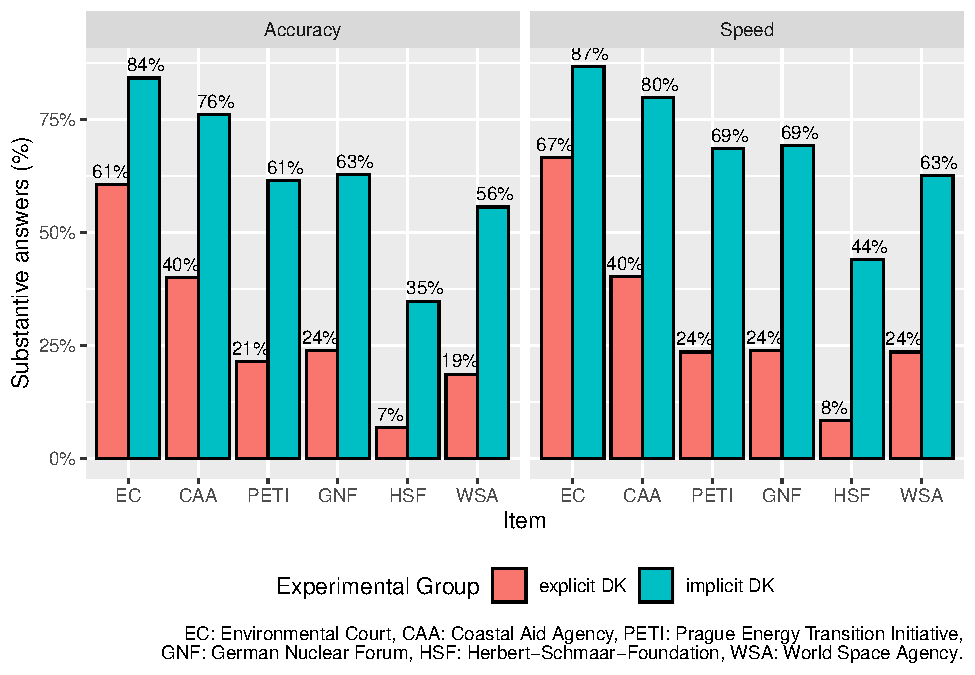
\includegraphics[width=1\linewidth]{article_files/figure-latex/barchart-1} \caption{\label{fig:barchart2}Substantive answers to fictitious oganizations}\label{fig:barchart}
\end{figure}

Before discussing the results of the multivariate models, we first look
descriptively at the effects of the experiments on the percentage of
substantive responses, per item, see Figure \ref{fig:barchart2}. First
of all, the barchart shows that sizable percentages of respondents gave
substantive responses to our fictitious issues. For the first
item,\footnote{The order of the items was not randomized. This was an
  unfortunate decision in retrospect. Randomization has already been
  included in the follow-up study.} the percentages of substantive
responses were the highest, with over 80\% substantive responses in the
implicit ``don't know'' treatment. The effect of an explicit ``don't
know'' category, however, is striking: it often more than halved the
percentages of substantive responses to fictitious issues. At the same
time, even in the explicit ``don't know'' group, often upwards of 20\%
of respondents still gave substantive responses. Interestingly, the
speed vs.~accuracy instructions seem to have little effect on the
percentages of substantive responses. If we follow the logic layed out
above, that satisficers tend towards quick, heuristic-led substantive
responses, then we would expect the speed condition to increase
substantive responses. This is in fact what we observe, with slightly
higher percentages of substantive answers on most items in the ``speed''
treatment. However, the differences are small and the multivariate
regressions suggest they are on the edge of statistic significance, see
Table \ref{tab:results}.

Moving on to the regression models, we see in Model 1, which includes
the response latencies as well as group or cluster means for them, along
with the experimental conditions and item dummies, that the response
latency variable is negative but not significant. Remember, the
specification of the models means we can look at these like
item-specific deviations from the respondent's overall response latency,
which, for their part, are reflected in the group or ``cluster'' means.
The coefficient for the cluster means is negative and in fact
significant at the 5\% level. This tells us that respondents that tend
to answer more slowly on average (larger response latency), tend to give
less substantive responses. The effect is summarized in Figure
\ref{fig:rl-plotb},\footnote{The plots show the predicted probability of
  a substantive response when the experiment and item dummies are set to
  their reference level while the other continuous variables are set to
  their mean, see \citet{Luedecke2021}. For this reason, the intercepts
  displayed in the plots do not represent the intercepts implied in the
  regression output (which set the continuous variables to zero).} which
displays the predicted probabilities of a substantive response over the
(cluster) mean response latency in seconds. The effect is a first
indication in support of the idea that substantive responses are linked
to satisficing (fast responses). However, the results suggests these are
between-respondent effects: respondents that respond slower on average
tend to also give less substantive answers to fictitious issues. The
same cannot be said about the per-item deviations from these overall
speeds, shown in Figure \ref{fig:rl-plota}. While the basic trend is the
same, the standard errors are too large to classify the effect as
significant. What this means is that faster responses
\textit{relative to one's own typical speed} do not significantly
predict responses in this model.

The implicit ``don't know'' category has a strong, highly significant
effect on the probability of giving a substantive response. This
confirms the findings in Figure \ref{fig:barchart2}: the lack of a
``don't know'' category leads to substantially more substantive
responses. The speed instructions are significant, but only at the 5\%
level. The effect is positive and it thus confirms the impression from
Figure \ref{fig:barchart2}: asking respondents to answer quickly,
without much thought, increased substantive responses and supports our
hypothesis that satisficing leads to more pseudo opinions.

There is also substantial differences between the individual items, as
seen in Figure \ref{fig:barchart2}. The arguably most obscure fictitious
issue, the ``Herbert-Schmaar Foundation'' produced the least pseudo
opinions by far. Notice the other items tend to provide some vague clues
as to the goals or motivation of the supposed organization. E.g.,
``Environmental Court'' obviously has something to do with the
environment. One could plausibly assume it has something to do with
environmental protection; perhaps it is a body for prosecuting those who
damage the environment. The ``Herbert-Schmaar Foundation'' provides no
such obvious clues. There may exist a number of people with the name
Herbert Schmaar, but to our knowledge there is no widely known person
with that name.

Moving on to model 2, where we introduce the squared response latency
terms, we see the main effect of response latencies is negative and
significant at the 5\% level, while the squared term is positive and
marginally significant. The predicted probabilities based on these
effects are shown in Figure \ref{fig:rl-plot2a}. The effects of the
response latency cluster means echo this in Model 2, shown in Figure
\ref{fig:rl-plot2b}. Now we have a highly significant negative main
effect, as well as a highly significant positive squared term. These
findings provide even clearer support for the idea that satisficers
(fast) tend to substantive responses, presumably in order to avoid
quality-control measures, while optimizers (slow) tend to also provide
substantive responses, presumably because the process of ``imputing a
meaning'' takes time and effort. The fact that the within-effects are
also approaching significance in Model 2 tells us, firstly, that faster
than average responses for a given person tend to predict a substantive
response to a ficitious issue. On the other hand, slower than average
response also tend to predict substantive responses to ficititous
issues. The effects of the other variables are largely stable compared
to Model 1.

Finally, in Model 3, we introduce the respondent-level variables in an
explorative step. Notice the sample size decreases dramatically from
Model 2 to Model 3 because of missings on the respondent-level
variables. For this reason, we prefer to interpret the response latency
effects from Model 2. In Model 3, the coefficients are largely the same
(as they should be: correlations between the response latencies and the
stable person-specific characteristics have already been eliminated
using the correlated random effects model), but the smaller sample size
causes a loss of power, and some of the effects fall out of
significance. Somewhat surprisingly, very few of the respondent-level
predictors have significant effects on the response behaviour. Males
tend to give more substantive responses to fictitious issues than women,
so too do older respondents, although these effects are significant only
at the 10\% level. Interestingly, political interest has a positive
highly significant effect on substantive responses: the more politically
interested the respondent claimed to be, the more substantive responses
to our ficitious issues they tended to give. This echos the findings of
\citet{Sturgis2010}, who found also found a significant positive
relationship between political interest and pseudo opinions. There, they
speculated that those susceptible to social desirability bias tend to
inflate their positive characteristics, and so self-reported political
interest predicted pseudo opinions because these respondents desired to
look knowledgeable in all domains, even on fictitious topics.
Puzzlingly, the need for social approval item has no discernible effect
on pseudo opinions. However, the need for social approval scale used
here was a compromise solution to a larger 16 item scale that did not
work as intended. Perhaps the measure of political interest here is a
more valid measure of one's need for social approval than the index we
used here.

\begin{table}
\caption{Correlated random effects probit regression models. DV: substantive responses.}
\begin{center}
\begin{small}
\begin{threeparttable}
\begin{tabular}{l D{)}{)}{9)3} D{)}{)}{9)5} D{)}{)}{9)5}}
\toprule
 & \multicolumn{1}{c}{Model 1} & \multicolumn{1}{c}{Model 2} & \multicolumn{1}{c}{Model 3} \\
\midrule
(Intercept)                    & 0.54 \; (0.13)^{***}  & 1.09 \; (0.19)^{***}   & 1.46 \; (1.04)          \\
Response latencies (RL)        &                       &                        &                         \\
\quad RL                       & -0.01 \; (0.01)       & -0.04 \; (0.02)^{*}    & -0.04 \; (0.02)^{\circ} \\
\quad Group (id) mean RL       & -0.06 \; (0.03)^{*}   & -0.37 \; (0.09)^{***}  & -0.35 \; (0.11)^{**}    \\
Experiments                    &                       &                        &                         \\
\quad Implicit don't know      & 1.45 \; (0.08)^{***}  & 1.45 \; (0.08)^{***}   & 1.55 \; (0.09)^{***}    \\
\quad Speed instructions       & 0.17 \; (0.08)^{*}    & 0.18 \; (0.08)^{*}     & 0.14 \; (0.09)          \\
Items (Ref.: EC)               &                       &                        &                         \\
\quad CAA                      & -0.69 \; (0.06)^{***} & -0.70 \; (0.06)^{***}  & -0.77 \; (0.08)^{***}   \\
\quad PETI                     & -1.34 \; (0.07)^{***} & -1.34 \; (0.07)^{***}  & -1.45 \; (0.08)^{***}   \\
\quad GNF                      & -1.30 \; (0.07)^{***} & -1.31 \; (0.07)^{***}  & -1.40 \; (0.08)^{***}   \\
\quad HSF                      & -2.35 \; (0.07)^{***} & -2.37 \; (0.07)^{***}  & -2.54 \; (0.09)^{***}   \\
\quad WSA                      & -1.51 \; (0.07)^{***} & -1.52 \; (0.07)^{***}  & -1.59 \; (0.08)^{***}   \\
Squared RL                     &                       &                        &                         \\
\quad RL$^2$                   &                       & 0.00 \; (0.00)^{\circ} & 0.00 \; (0.00)          \\
\quad Group (id) mean RL$^2$   &                       & 0.04 \; (0.01)^{***}   & 0.03 \; (0.01)^{**}     \\
Respondent-related variables   &                       &                        &                         \\
\quad Male                     &                       &                        & 0.18 \; (0.09)^{\circ}  \\
\quad Age                      &                       &                        & 0.01 \; (0.00)^{\circ}  \\
\quad Need for social approval &                       &                        & -0.00 \; (0.02)         \\
\quad Political interest       &                       &                        & 0.21 \; (0.05)^{***}    \\
\quad Political orientation    &                       &                        & 0.01 \; (0.02)          \\
\quad Motivation               &                       &                        & 0.03 \; (0.02)          \\
\quad Opportunity              &                       &                        & -0.05 \; (0.05)         \\
\quad Education low            &                       &                        & 0.01 \; (0.10)          \\
\quad Lied                     &                       &                        & 0.02 \; (0.22)          \\
\quad Finished                 &                       &                        & -0.38 \; (1.02)         \\
\midrule
AIC                            & 7259.22               & 7239.48                & 5063.48                 \\
BIC                            & 7335.62               & 7329.77                & 5215.37                 \\
Log Likelihood                 & -3618.61              & -3606.74               & -2508.74                \\
Num. obs.                      & 7676                  & 7676                   & 5453                    \\
Num. groups: id                & 1287                  & 1287                   & 914                     \\
Var: id (Intercept)            & 1.56                  & 1.53                   & 1.27                    \\
\bottomrule
\end{tabular}
\begin{tablenotes}[flushleft]
\tiny{\item $^{***}p<0.001$; $^{**}p<0.01$; $^{*}p<0.05$; 
                           $^{\circ}p<0.1$. Two-tailed test. 
                           \item EC: Environmental Court, CAA: Coastal Aid Agency, PETI: Prague Energy Transition Initiative, GNF: German Nuclear Forum, HSF: Herbert-Schmaar-Foundation, WSA: World Space Agency.}
\end{tablenotes}
\end{threeparttable}
\end{small}
\label{tab:results}
\end{center}
\end{table}

\begin{figure}
\subfloat[\label{fig:rl-plota}Response latencies\label{fig:unnamed-chunk-4-1}]{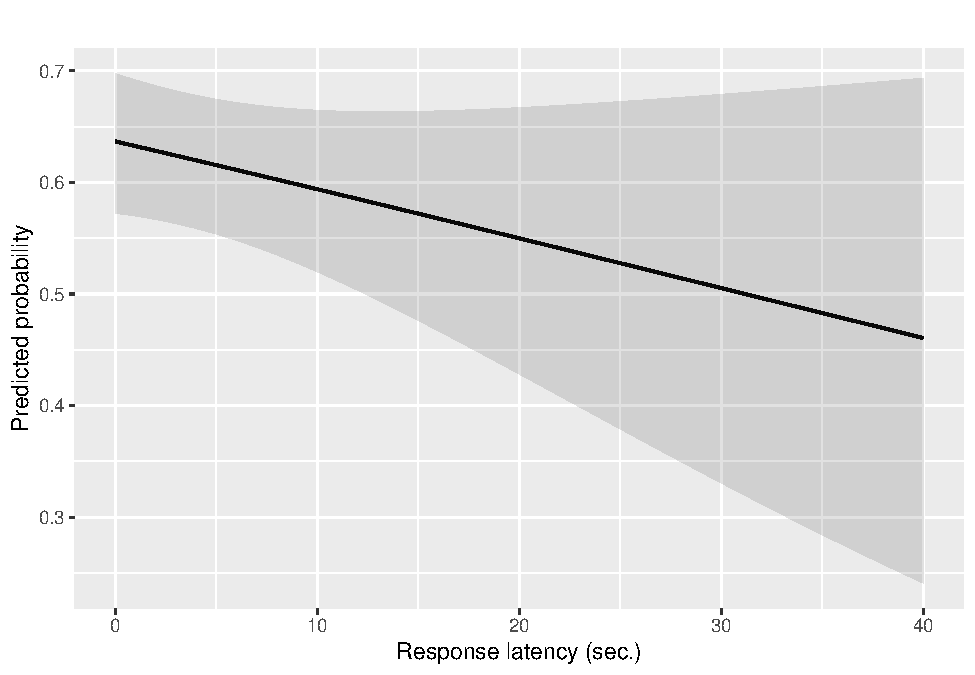
\includegraphics[width=0.5\linewidth]{article_files/figure-latex/unnamed-chunk-4-1} }\subfloat[\label{fig:rl-plotb}Group (id) mean response latencies\label{fig:unnamed-chunk-4-2}]{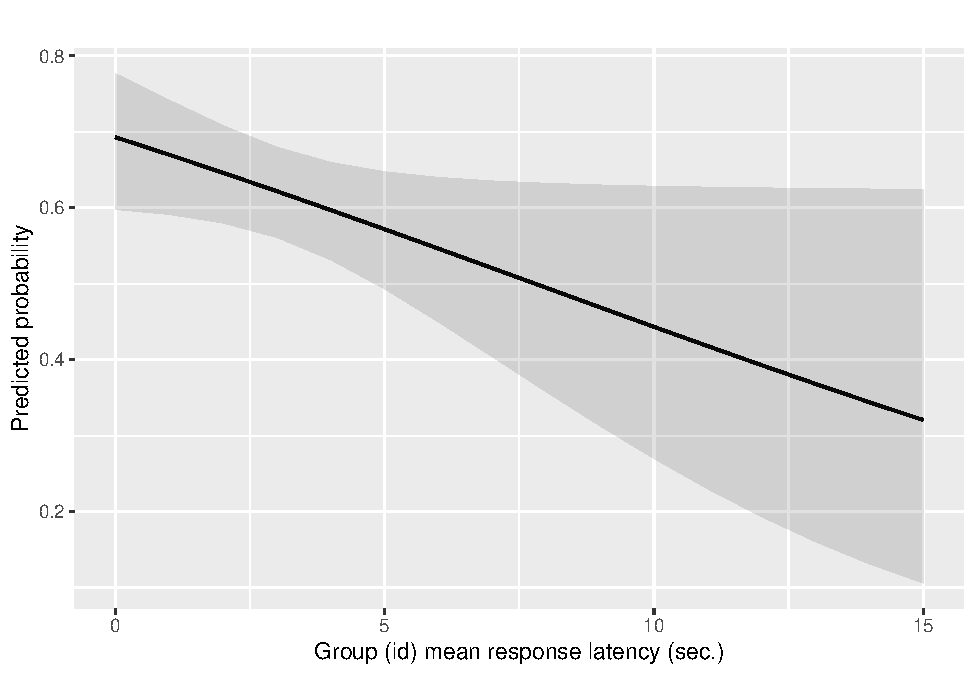
\includegraphics[width=0.5\linewidth]{article_files/figure-latex/unnamed-chunk-4-2} }\caption{\label{fig:rl-plot}Predicted probability of substantive response over response latencies (Model 1)}\label{fig:unnamed-chunk-4}
\end{figure}

\begin{figure}
\subfloat[\label{fig:rl-plot2a}Response latencies\label{fig:unnamed-chunk-5-1}]{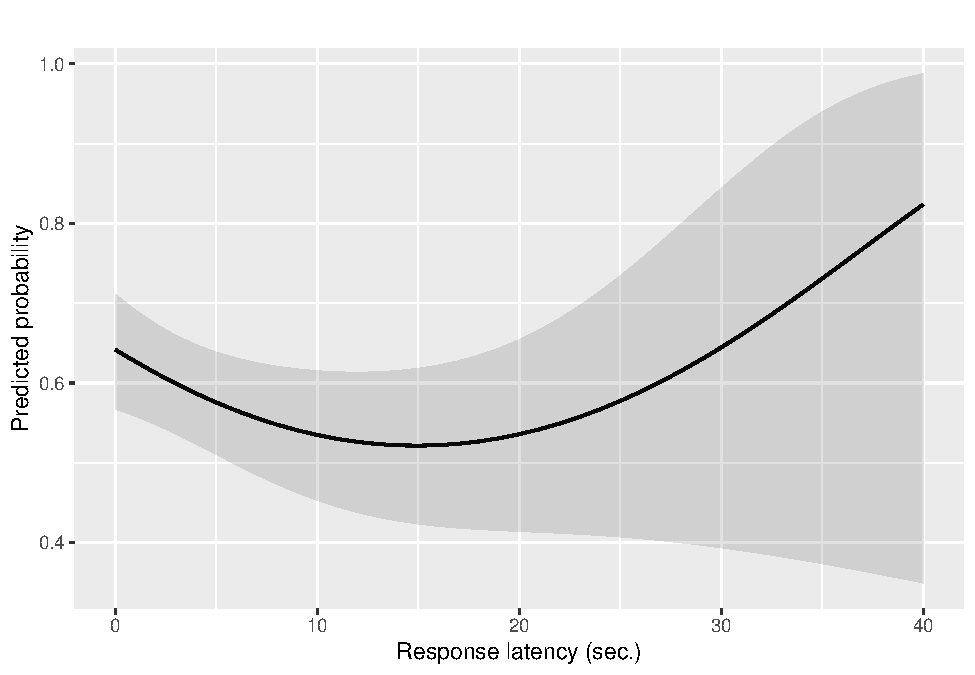
\includegraphics[width=0.5\linewidth]{article_files/figure-latex/unnamed-chunk-5-1} }\subfloat[\label{fig:rl-plot2b}Group (id) mean response latencies\label{fig:unnamed-chunk-5-2}]{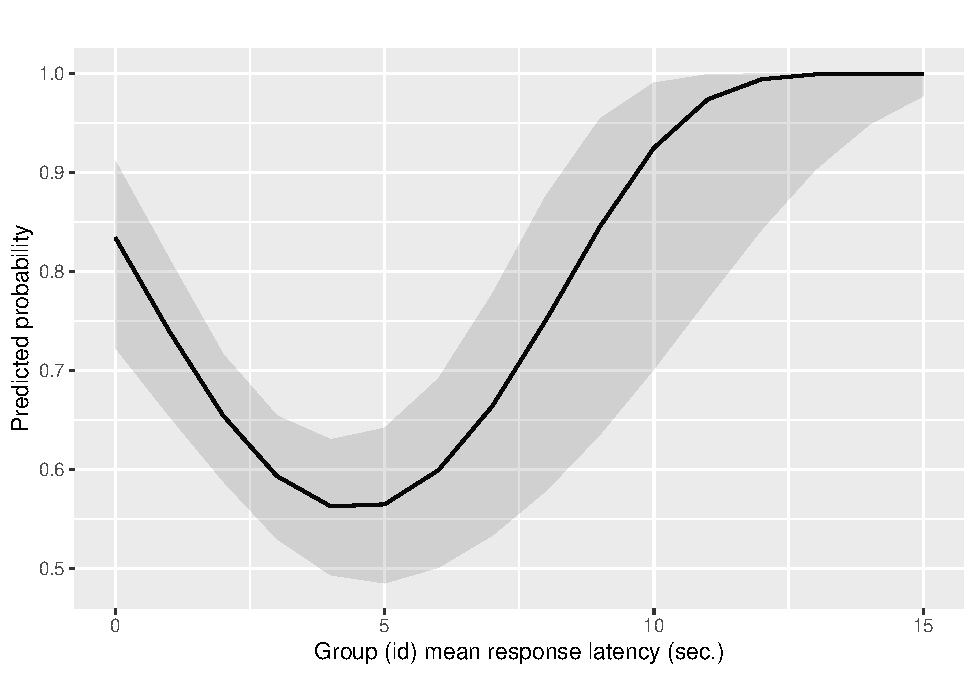
\includegraphics[width=0.5\linewidth]{article_files/figure-latex/unnamed-chunk-5-2} }\caption{\label{fig:rl-plot2}Predicted probability of substantive response over response latencies (Model 2)}\label{fig:unnamed-chunk-5}
\end{figure}

\hypertarget{conclusion-and-discussion}{%
\section{Conclusion and discussion}\label{conclusion-and-discussion}}

xxx

\bibliographystyle{sageh}
\bibliography{references}


\end{document}
